\section{Finite-Sample Behavior}
\label{sec:numerical}
\label{sec:finite-sample}

The population results imply that a one-factor model can meet a conventional fit cutoff while representing two traits, and that its loading pattern can depend on the estimator and the initial values. A finite-sample study examined both consequences; Appendix~\ref{supp:numerical} gives its details, and Appendix~\ref{app:binary} shows that the population transition also appears with binary items.

The design crossed 92 populations, four sample sizes (250, 500, 1,000 and 2,000), and three response formats (continuous, and four categories with symmetric or skewed thresholds), yielding 1,104 cells: exchangeable blocks of 4 or 8 items per trait with loading .5 or .7 (Design A), two four-item blocks with loadings .68 and .72 or .60 and .80 (Design B), and the PHQ-ADS layout of 9 and 7 items with loading .75 (Design C). Trait correlations ran from 0 to .9 in steps of .1, plus .01, .24 and .409 in Design B and further design-specific values in Designs A and C. One-factor models were fitted in lavaan (Rosseel, 2012) by ML, ULS, WLSMV and ML on ordinal scores; in Designs B and C at $N=500$ and 2,000, the ML fits also used both default item orders and 20 random starts (Appendix~\ref{supp:design}). A solution group is higher-objective when its lavaan objective exceeds that of the \emph{best solution found}, the group with the lowest observed objective, by more than $10^{-7}$; these classifications do not establish sample stationarity or global optimality.

Loading imbalance was summarized by the magnitude contrast $M=|\bar l_A|-|\bar l_B|$ between the block means of the standardized loadings and by the normalized magnitude contrast $C_{\mathrm{mag}}$ defined in Appendix~\ref{supp:design}. These quantities describe loading patterns; they are not factor-score estimates.

\subsection{Fit Indices}

Sample fit indices generally followed their population references (best-found multistart solutions, checked against the closed forms where available), although the agreement depended on the solution returned. In Designs A and C, the correlation at which half the samples met CFI $\ge.95$ or RMSEA $\le.06$ was within .03 of the population crossing point at every sample size, whereas for SRMR at $N=250$ the correlation required to pass the cutoff was up to .11 higher than the population value (Appendix~\ref{supp:fit}). For ordinal items, the population reference values of robust WLSMV CFI, TLI and RMSEA (Savalei, 2021) were within .004 of the continuous-ML population values across the evaluated populations with $\varphi\ge.7$, a numerical finding for these designs, whereas lavaan's unscaled and scaled WLSMV indices were more lenient near the cutoffs. The population agreement did not eliminate differences in small-sample cutoff-passing rates: in the PHQ-ADS layout at $N=250$ and $\varphi=.912$, robust WLSMV CFI passed less often than continuous-ML CFI, 83\% against 99\%.

\subsection{Loading Imbalance and Item Order}

The estimators differed substantially in the magnitude of sample loading imbalance (Figure~\ref{fig:4}). With four items per trait, loading .7 and $N=2{,}000$, mean $|C_{\mathrm{mag}}|$ under ML declined from .930 at $\varphi=0$ to .139 at the grid point .409 near $\varphi^*$ and .048 at .5. Under ULS, it was .317 at the ULS population threshold $1/p=.125$, and WLSMV on symmetric categories produced much less imbalance, .102 at $\varphi=0$. Thus, the population thresholds locate changes in the population solution, but sample imbalance remains positive on both sides (Appendix~\ref{supp:imbalance}).

\begin{figure}[t]
\centering
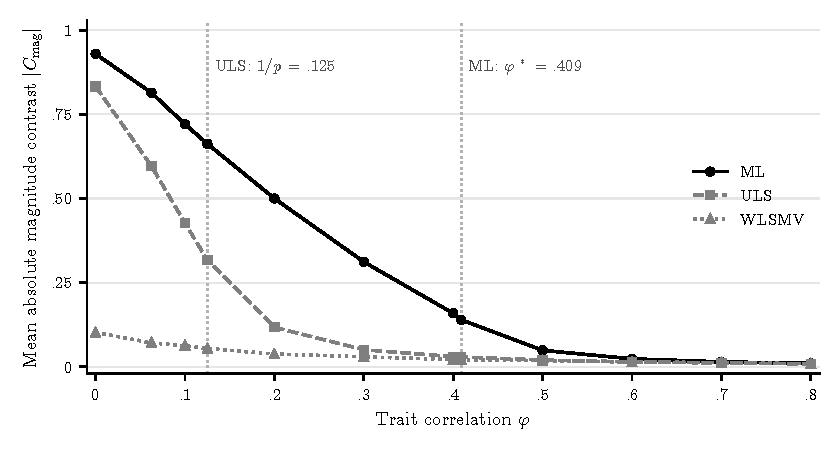
\includegraphics[width=0.85\textwidth]{fig4.pdf}
\caption{Mean absolute normalized magnitude contrast $|C_{\mathrm{mag}}|$ of one-factor fits, with 4 items per trait, loading .7 and $N=2{,}000$; WLSMV on four symmetric categories. Each point averages 1,000 continuous fits or 500 ordinal fits with valid contrasts; Monte Carlo standard errors are at most .005. The evaluated correlation $\varphi=.9$ (values below .01) is not shown. Dotted lines mark the population ML threshold $\varphi^*=.409$ and ULS threshold $1/p=.125$. Magnitudes do not encode polarity: at $\varphi=0$, opposite block signs occur in 510/1,000 ML and ULS fits and 257/500 WLSMV fits. At .0625 the counts are 15/1,000, 15/1,000 and 14/500; above .0625 they are zero on this grid.}
\label{fig:4}
\end{figure}

Item order was associated with which trait the fitted factor represented. In Design A, the two population minima below the ML threshold are mirror images, yet among default fits with $|M|>.1$ at $N=2{,}000$, the proportion with $M>.1$, favoring the first-listed block, was 86\% for continuous ML, 85\% for ML on scores, 68\% for ULS and 56\% for WLSMV (Figure~\ref{fig:5}, right). These pooled proportions are conditional on a descriptive selection, not a calibrated test. Their direction is consistent with lavaan's default starting values, which are anchored on the first-listed item.

\begin{figure}[t]
\centering
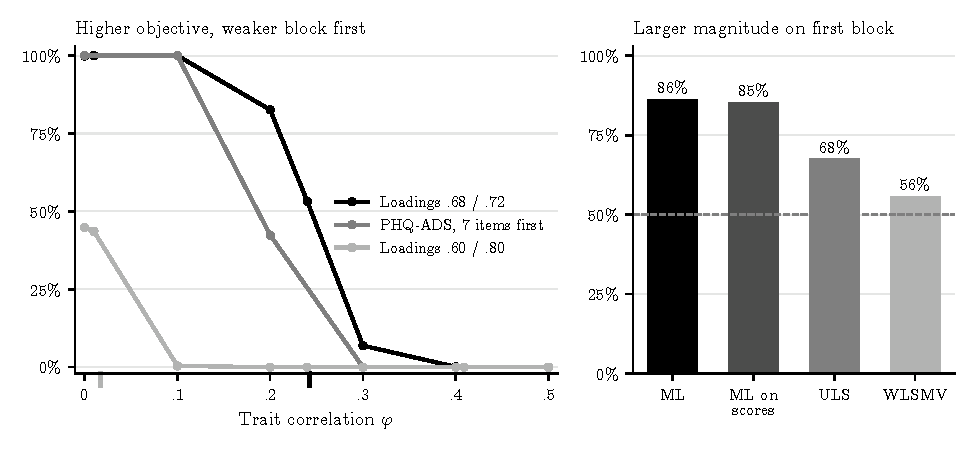
\includegraphics[width=\textwidth]{fig5.pdf}
\caption{Item order and lavaan's default start, $N=2{,}000$. Left: share of continuous ML fits assigned to a higher-objective solution group that follows the weaker block when that block is listed first. Each point uses 1,000 archived replications. Ticks mark the two Design B population folds. Right: pooled share of magnitude-selected fits ($|M|>.1$) with $M>.1$ in the exchangeable design, over all four conditions and their complete correlation grids. ML and ULS use continuous items; ML on scores and WLSMV use symmetric four-category items. Selected/attempted fits are 28,719/53,000 (ML), 13,501/26,500 (ML on scores), 18,344/53,000 (ULS) and 4,746/26,500 (WLSMV); the pooled shares are dominated by low-correlation cells, where $|M|>.1$ is common. The dashed line is the 50\% reference. Solution groups do not certify sample minima.}
\label{fig:5}
\end{figure}

When the blocks differed, item order could also lower the fit reported from the default start (Figure~\ref{fig:5}, left; Table~\ref{tab:4}). With the weaker block listed first, continuous ML returned a higher-objective group favoring that block in 94 to 100\% of samples at $\varphi\le.1$ and $N=500$ and 2,000, both with loadings .68 and .72 and in the PHQ-ADS layout with the 7-item block first. Listing the weaker block last produced no weaker-block flags in the 234 archived cell--analysis combinations, although 761 of the 156,000 multistart replications retained a higher-objective group under that order. In the PHQ-ADS layout with depression items listed first, the default-order weaker-block flag was absent in these simulations; that result does not establish which solution was obtained in the published trials.

\begin{table}[t]
\centering\small
\caption{Continuous ML in Designs B and C: population reference CFI, mean sample CFI, and the frequency of higher-objective weaker-block solutions. Default starts use design order: the weaker block first in Design B and the stronger block first in Design C. Each sample entry uses 1,000 paired replications; Monte Carlo standard errors of the percentages are at most 1.6 percentage points. The best solution found is the retained solution group with the lowest observed objective. Its CFI is reconstructed using the estimated baseline noncentrality; all 18,000 pairs satisfy the inversion domain. Population entries are best-found numerical reference values from multistart fitting; no closed form applies to these designs.}
\label{tab:4}
\setlength{\tabcolsep}{3pt}
\begin{tabularx}{\textwidth}{@{}>{\raggedright\arraybackslash}p{3.7cm}c*{5}{>{\centering\arraybackslash}X}>{\centering\arraybackslash}p{2.1cm}@{}}
\toprule
Design and order & $\varphi$ & Population CFI & Default start, $N = 500$ & Default start, $N = 2{,}000$ & Best found, $N = 500$ & Best found, $N = 2{,}000$ & Higher-objective weaker group, $N = 500$ / 2,000 \\
\midrule
.68 and .72, weaker first & 0 & .558 & .443 & .442 & .561 & .559 & 95\% / 99.9\% \\
.68 and .72, weaker first & .1 & .567 & .460 & .454 & .568 & .567 & 94\% / 100\% \\
.68 and .72, weaker first & .2 & .591 & .538 & .513 & .595 & .592 & 65\% / 83\% \\
.68 and .72, weaker first & .24 & .606 & .571 & .563 & .607 & .606 & 49\% / 53\% \\
.68 and .72, weaker first & .3 & .632 & .618 & .630 & .632 & .633 & 26\% / 7\% \\
.60 and .80, weaker first & 0 & .767 & .630 & .533 & .767 & .766 & 28\% / 45\% \\
.60 and .80, weaker first & .1 & .771 & .731 & .768 & .768 & .770 & 8\% / 0.4\% \\
PHQ-ADS layout, stronger first & 0 & .585 & .585 & .585 & .585 & .585 & 0\% / 0\% \\
PHQ-ADS layout, stronger first & .1 & .590 & .590 & .590 & .590 & .590 & 0\% / 0\% \\
\bottomrule
\end{tabularx}
\end{table}

Higher-objective weaker-block groups also occurred above the population fold (Table~\ref{tab:4}, $\varphi=.3$) and have no sample stationarity certificate. In all 156,000 archived multistart replications, at least one default-order group was within $10^{-7}$ in lavaan objective of the best group found with the additional random starts, so checking both item orders was useful in this study; this result concerns the evaluated designs and retained groups and does not guarantee global optimality.
